% last update 13 jan 2021
% last update 27 dec 2020
% first release 11 dec 2020
% reviewed version 3 dec 2020

% EQUATION LIST
% FOURIER TRANSFORM: 
% x(t) = \frac{1}{2 \pi} \ \int_{-\infty}^{+\infty} \ X( \omega) \ e^{j \omega t} \ d\omega

% INVERSE FOURIER TRANSFORM:
% X(\omega) =  \int_{-\infty}^{+\infty} x(t) \ e^{-j \omega t} \ dt

%FOURIER SERIES
% x(t) =  \sum_{k=-\infty}^{\infty} \ c_{k} \ e^{j\frac{2\pi k}{T}t} 
% c_{k} = \frac{1}{T} \int_{0}^{T} x(t) \ e^{-j\frac{2\pi k}{T}t} 


\documentclass[12pt,a4paper]{article}

\usepackage[utf8]{inputenc}
\usepackage[english]{babel}

\usepackage{subfigure}
 
\usepackage{tikzducks}

\usepackage{hyperref}
\hypersetup{hidelinks}
\hypersetup{pdfauthor={Li, Binghuan},
            pdftitle={Signals and Control II},
            }

\usepackage[margin=2.5cm]{geometry}
\usepackage{wrapfig}
\usepackage{graphicx}
\usepackage{fancyhdr}
\usepackage{xcolor}

\usepackage{amsmath}
\usepackage{amsfonts}
\usepackage{mathrsfs} 
\usepackage{mathtools} 
\usepackage{amssymb}

\usepackage[font={small,it}]{caption}
\captionsetup[figure]{labelfont={sc},name={Fig.}}

\usepackage{float}

\usepackage{tcolorbox}
\tcbuselibrary{breakable}

\usepackage[european]{circuitikz}
\usepackage{tikz}
    \usetikzlibrary{arrows}

\usepackage{tabularx}

\usepackage{sidecap}

\usepackage{cancel}
%----------Footer & Header----------%
\pagestyle{fancy}
\fancyhf{}
\lhead{\textit{\leftmark}}
\lfoot{\textbf{\thepage}}%LEFT foot page number

%----------Define \doublerule command----------%
\newcommand{\doublerule}[1][.4pt]{% <===================================
  \noindent
  \makebox[0pt][l]{\rule[.7ex]{0.8\linewidth}{#1}}%
  \rule[0.4pt]{0.8\linewidth}{#1}\par} % <============
  
%----------BEGIN----------%
\begin{document}

%----------Title page----------%
\begin{titlepage}
\newgeometry{margin=2.5cm}
  \begin{center}
  \begin{minipage}{0.15\textwidth}
    \includegraphics[width=2.3\textwidth]{images/Imperial.eps}%IMPERIAL LOGO
  \end{minipage}
  \hspace{22pt}
  \begin{minipage}{0.7\textwidth}
    \raggedleft \bfseries
    Department of Bioengineering\\Biomedical Engineering\\
   \doublerule{Lecturer: \emph{Prof.} Dario Farina}
     \end{minipage}
\end{center}
\vspace{3.5cm}
{\centering
  {\huge\bfseries Signals and Control II \par}%MAIN TITLE
    \vspace{1cm}
  {\huge\bfseries Signals\par}
    \vspace{3cm}
  
\begin{tikzpicture}%DUCK PIC
  \duck[graduate=gray!20!black,
      tassel=red!70!black]
\end{tikzpicture}\\
  \vspace{3cm}
  {\scshape\Large Year 2\par}%SUBTITLE
  {\scshape\Large2020, Autumn Term\par}%SUBTITLE
  }
\vspace{4cm} 
\hrule
\vspace{0.5cm}
\begin{minipage}[b]{0.35\linewidth}
\large{\underline{\textbf{Author:}}}\\
\textsc{\href{mailto:binghuan.li19@imperial.ac.uk}{Binghuan Li}}
 \end{minipage}
 \hfill
\begin{minipage}[b]{0.35\linewidth}
\large{\underline{\textbf{Last Update:}}}\\
\textsc{\today}
 \end{minipage}
 \vspace{0.5cm}
\hrule

\end{titlepage}

%----------DO NOT CHANGE THE SETTINGS ABOVE----------%
\newpage
\section*{Acknowledgement}
I would like to express my deepest appreciation to \emph{Prof. Dario Farina} for his help in reviewing these notes with the highest profession.
\ \\ \\
I would like to extent my sincere thanks to \emph{Rea Tresa}, \emph{Ben Ford}, and \emph{Elisa Soliani} for their insightful comments. Their work significantly optimized the structure. 
\ \\ \\
Special thanks to \emph{Haroon Chughtai}. His notes greatly enlightened me when preparing this new set.

\vspace{1cm}
\section*{Update Notes}
\subsection*{13$^{th}$ Jan, 2021}
\begin{enumerate}
\item  \emph{Section 3.5.3}: Corrected typos: missing comma in $<f_{1}(t), f_{2}(t)>$.
\item \emph{Section 5.3.8}: Corrected math typos in the derivation: missing $d\tau$ in line 1, $d\tau \to d\alpha$ in line 3.
\item \emph{Section 5.3.8}: Corrected typos: missing $\omega_{0}$ in $\cos(\omega_{0} t)$.
\item \emph{Section 5.6}: Added the formula for finding the phase angle. Added a plot for $sign(x)$.
\end{enumerate}
\subsection*{27$^{th}$ Dec, 2020}
\begin{enumerate}
\item \emph{Section 5.3.2}: Added the derivation of time shifting property.
\item \emph{Section 5.5}: Corrected math typos, rearranged the example and improved the readability.
\item \emph{Section 5.5.1}: Added a description of LTI systems.
\item \emph{Section 5.6}: Refined the description of magnitude and phase spectra. An example is adopted from the textbook.
\end{enumerate}


\newpage
\tableofcontents%INDEX

%==============================================%

%----------Definition, Classification and Properties of Signals----------%
\newpage
\section{Definition, Classification and Properties of Signals}
\subsection{Definition of signals}
 \begin{itemize}
 \item  Signals describe physical phenomena as patterns of variations of some form.
 \item Mathematically, signals are \textbf{functions} of one or more independent variables.
 \item For example, a signal $s(t)$ can be a function of the continuous independent variable time $t \in [\alpha, \beta]$ A two-dimensional signal $f(x, y)$ can be a function of two spatial coordinates $x, y$.
 \end{itemize}

\subsection{Continuous and Discrete-time Signals}
 \begin{itemize}
 %\item We focus on the signals of one independent variable. Without loss of generality, we will choose this independent variable to be time $t$.
 \item Signals can be a function of the \textbf{continuous time} variable, in which case we will use the notation $x(t)$ with $t \in \mathbb{R}$, \\
or of the \textbf{discrete time} variable, in which case we will use the notation $x[n]$ with $n \in \mathbb{Z}$. (\textsc{Fig.1})

 
 \begin{figure}[H]
 \begin{minipage}{0.5\textwidth}
  \includegraphics[width = \textwidth]{images/continuous_signals}
  \end{minipage} \hfill
  \begin{minipage}{0.5\textwidth}
  \includegraphics[width=\textwidth]{images/discrete_signals}
  \end{minipage}
  \caption{Continuous signal $x(t)$ and discrete signal $x[n]$ }
 \end{figure}
 
 \item Discrete-time signals are often (but not necessarily) a sampling of continuous-time signals.
 \[ x[n] = x_{c}(nT) \quad -\infty < n < +\infty \]
 \ $T$ is sampling period.
 \item A discrete-time signal can be represented as a sequence of numbers, or, a vector.
 \end{itemize}

 \subsubsection{Digital Signals}
 \begin{itemize}
 \item When we speak of a digital signal we often mean one that has been \textbf{sampled} (captured at regular points in time) and \textbf{quantisised}.
 \item When one refers to a 12-bit signal, they are referring to the number of amplitude quantisation levels.
 \item Sampling a continuous signal may be done \textbf{without losing any information} from the original signal. Conversely, quantisation always implies \textbf{losing information}. (\textsc{Fig.2})
 \end{itemize}
 \begin{figure}[h!]\centering
  \includegraphics[width = 0.6\textwidth]{images/1.2.1}
  \caption{Sampling and quantisation}
 \end{figure}
 \textit{We focus on the signals of one independent variable!}
 
\subsection{Deterministic and Stochastic Signals}
 \begin{itemize}
 \item \textbf{Deterministic}: a signal that \textbf{can be predicted} exactly (an analytical formulation exists). 
 \begin{itemize}
  \item Example: $x(t) = \sin(2\pi t)$
  \end{itemize}
 \item \textbf{Stochastic}: a signal that \textbf{cannot be predicted} exactly before it has “occurred”; any signal that conveys information to us when we observe it. 
  \begin{itemize}
  \item Example: Thermal noise across a resistor, EEG traces, etc.
  \end{itemize}
 \item We can often meaningfully describe the statistical properties of stochastic signals by building a model of their generation (stochastic processes).
 \end{itemize}
\textit{We will mainly deal with deterministic signals in this course!}

\subsection{Periodic Signals}
 \begin{itemize}
 \item A periodic continuous-time signal $x(t)$ has the property that there is a positive value of $T$ for which $x(t) = x(t+T)$ for all values of $t$ (similar definition for discrete-time signals).
 \item A periodic signal has the property that it is unchanged by a time shift of $T$, we will say that $x(t)$ is periodic with period $T$. (\textsc{Fig.3})
 \end{itemize}
 \begin{figure}[H]\centering
 \includegraphics[width = 0.6\textwidth]{images/1.5}
 \caption{A periodic signal with period $T$}
 \end{figure}

\subsection{Signal Energy and Power}
For a continuous-time signal $x(t)$ for $t_1 \leq t \leq t_2$ and for a discrete-time signal $x[n]$ for $n_1 \leq n \leq n_2$, energy and power can be represented as follows:
\[ \text{Energy(continuous time)} = \int_{t_1}^{t_2} \lvert x(t) \rvert^2 \ dt \]
\[ \text{Power(continuous  time)} = \frac{1}{t_2 - t_1} \ \int_{t_1}^{t_2} \ \lvert x(t) \rvert^2 \ dt \]
\[ \text{Energy(discrete time)} = \sum_{n_1}^{n_2} \ \lvert x[n] \rvert ^2 \]
\[ \text{Power(discrete time)} = \frac{1}{n_2 - n_1} \sum_{n_1}^{n_2} \ \lvert x[n] \rvert ^2 \]

\begin{tcolorbox}[breakable]
 %\underline{\textsc{Derivation}}\\
  We get the conclusion above from the calculation for electrical power and energy.
  Let $v(t)$ and $i(t)$ represent the voltage and current across the resistor of resistance $R$. 
 \begin{itemize}
  \item The instantaneous power across the resistor is the product $v(t)i(t)$, which is proportional to $v^2(t)$.
  \item The total energy \[ \int_{t_1}^{t_2} \ \frac{1}{R} \ v^2(t) \ dt \] 
  \item The average power \[ \frac{1}{t_2 - t_1} \ \int_{t_1}^{t_2} \ \frac{1}{R} \ v^2(t) \ dt \]
  \end{itemize}
  Similar properties can be applied to any continuous-time signals and discrete-time signals.
\end{tcolorbox}
  
\begin{itemize}
 \item Often, the signals are directly related to physical quantities capturing power and energy in a physical form.
 \item These properties are important characteristics of signals, even if in some cases do not reflect physical energy or power.
 %\item Therefore, we extend the above definition of energy and power to any continuous-time signal as well as discrete-time signal (including the case of complex signals)
\end{itemize}

\subsubsection{Energy and Power of a Generic Signal}
%We extend the previous definition to any continuous-time signal $x(t)$ for $t_1 \leq t \leq t_2$ and and discrete-time signal $x[n]$ for $n_1 \leq n \leq n_2$, as follows:
%\[ Energy(continuous \ time) = \int_{t_1}^{t_2} \lvert x(t) \rvert^2 \ dt \]
%\[ Power(continuous \ time) = \frac{1}{t_2 - t_1} \ \int_{t_1}^{t_2} \ \lvert x[n] \rvert^2 \ dt \]
%\[ Energy(discrete \ time) = \sum_{n_1}^{n_2} \ \lvert x[n] \rvert ^2 \]
%\[ Power(discrete \ time) = \frac{1}{n_2 - n_1} \sum_{n_1}^{n_2} \ \lvert x[n] \rvert ^2 \]
Extend the range to: $-\infty<t<+\infty$ or $-\infty<n<+\infty$ 
\begin{itemize}
 \item In continuous time:
  \[ \text{Energy}= \int_{-\infty}^{+\infty} \ \lvert x(t) \rvert^2 \ dt \]
  \[ \text{Power}= \lim_{T \to \infty} \ \frac{1}{2T} \ \int_{-T}^{T} \ \lvert x(t) \rvert^2 \ dt \]
 \item In discrete time:
  \[ \text{Energy}= \sum_{-\infty}^{+\infty} \ \lvert x[n] \rvert^2 \]
  \[ \text{Power}=\lim_{N \to +\infty} \ \frac{1}{2N+1} \ \sum_{-N}^{N} \ \lvert x[n] \rvert^2 \]
\end{itemize}
\textit{We will use the mathematical definitions above, regardless of the direct physical meaning of each term!}

%----------------Test Signals----------------%
\newpage
\section{Types of Signals}

%----------------complex exp in ct----------------%
\subsection{Periodic Complex Exponential Signals in Continuous-time Domain}

 \[ x(t) = e^{j\omega_0 t} \]
\begin{itemize}
 \item Periodic, period $T = \frac{2\pi}{\lvert \omega_0 \rvert}$.
 \item The signal $x(t) = e^{-j\omega_o t}$ has the same period.
 \item The complex exponential defined above is closely related to the sinusoidal signal:
 \[ x(t) = A \cos(\omega_0 t + \phi) = \frac{A}{2} e^{j\phi}e^{j \omega_0 t} +\frac{A}{2} e^{-j\phi}e^{-j \omega_0 t} \]
  \ which has the same period $T = \frac{2\pi}{\lvert \omega_0 \rvert}$.
 \item The complex exponentials and sinusoidal signals have \textbf{infinite energy} and \textbf{finite
  power}.
 \begin{itemize}
  \item Example: for the signal $x(t)= A \cos(2\pi \omega_{0}t+\phi)$ with the period $T_{1}$,
  \[ \text{Power} = \frac{A^{2}}{2} \]
 \end{itemize}
\end{itemize}

%----------------complex exp in dt----------------%
\subsection{Periodic Complex Exponential Signals in Discrete-time Domain}

 \[ x[n] = e^{j\omega_0 n} \]
 \ And the sinusoidal signal becomes 
 \[ x[n] = A \cos(\omega_0 n + \phi) = \frac{A}{2} e^{j\phi}e^{j \omega_0 n} +\frac{A}{2} e^{-j\phi}e^{-j
  \omega_0 n} \]
 \begin{itemize}
  \item $n \in \mathbb{Z}$. Thus, $x[n]$ is the same signal for $\omega_0 + 2\pi k$ with $k \in
   \mathbb{Z}$. The frequency of oscillation in discrete time exponentials does not increase
   monotonically but is limited to $2\pi$.
  \item $x[n]$ is not always periodic.
 \end{itemize}
 
%----------------unit imp in dt----------------%
\subsection{The Unit Impulse in Discrete-time Domain}

In discrete-time domain, the \textbf{unit impulse} is the simplest signal: (\textsc{Fig.4})\\
\boxed{
 \begin{minipage}{0.3\textwidth}
   \[  \delta[n] = \begin{cases}
   1,&n=0\\
   0,&n\neq0
  \end{cases}\]
 \end{minipage} \
 \begin{minipage}{0.7\textwidth}
  \begin{figure}[H] \centering \includegraphics[width=0.7\textwidth]{images/1.6.1}
  \caption{The unit impulse} \end{figure}
 \end{minipage}
  }
  
The discrete-time signal impulse \textbf{delayed by the integer $k$} is as follows: (\textsc{Fig.5})\\
\boxed{
 \begin{minipage}{0.3\textwidth}
   \[ \delta[n-k] = \begin{cases}
   1,&n=k\\
   0,&n \neq k\\
  \end{cases}\]
 \end{minipage} 
 \begin{minipage}{0.7\textwidth}
  \begin{figure}[H]\centering \includegraphics[width=0.7\textwidth]{images/1.6.2}
  \caption{The unit impulse delayed by the integer $k$} \end{figure}
 \end{minipage}
}

\begin{itemize}
 \item For any discrete-time signal $x[n]$, directly from the definition of $\delta[n]$, we have
   \[ x[n] \ \delta[n-k] = x[k] \ \delta[n-k] \]
 \quad \textbf{This implies:} any signal multiplied by the unit impulse is zeroed for all time samples, apart from the integer
 time where the unit impulse is centered.
 \item From the property above, we have:
 \begin{align*} \begin{split}
  \sum_{n=-\infty}^{\infty}x[n]\delta[n-k]  &=  \sum_{n=-\infty}^{\infty}x[k] \ \delta[n-k] \\
  &= x[k] \cancelto{1, \text{when} \ k=n}{\sum_{n=\infty}^{\infty}\delta[n-k]} \\
  &= x[k]
 \end{split} \end{align*}
 \item Any arbitrary discrete-time signal can be expressed as the sum of \textbf{scaled} and \textbf{delayed} impulses:
 \[ x[n] = \sum_{k=-\infty}^{+\infty}x[k]\delta[n-k] \] 
\end{itemize}

%----------------unit imp in dt----------------%
\subsection{The Unit Step in Discrete-time Domain}
Unit step in discrete-time domain is defined as: (\textsc{Fig.6})\\
\boxed{
 \begin{minipage}{0.3\textwidth}
  \[u[n] = \begin{cases}
   1, & n\geq 0\\
   0, & n<0 \\
  \end{cases} = \sum_{k=0}^{+\infty}\delta[n-k] \]
 \end{minipage}
 \begin{minipage}{0.7\textwidth}
  \begin{figure}[H]\centering \includegraphics[width=0.7\textwidth]{images/1.6.3}
  \caption{Unit step in discrete-time domain} \end{figure}
 \end{minipage}
}
\begin{itemize}
 \item The unit impulse is the discrete time derivative of the unit step.
 \[ \delta[n] = u[n] - u[n-1] \]
\end{itemize}

%----------------unit step in ct----------------%
\subsection{The Unit Step in Continuous-time Domain} 
Unit step in continuous-time domain is defined as: (\textsc{Fig.7})\\
\boxed{
 \begin{minipage}{0.3\textwidth}
  \[ u(t) = \begin{cases}
   1, & t > 0\\
   0, & t < 0 \\
  \end{cases} \]
 \end{minipage}
 \begin{minipage}{0.7\textwidth}
  \begin{figure}[H]\centering \includegraphics[width=0.5\textwidth]{images/1.6.4}
  \caption{Unit step in continuous-time domain} \end{figure}
 \end{minipage}
}
\begin{itemize}
\item The continuous-time unit step function has a discontinuity in $t=0$, it is \textbf{not differentiable}. To solve the issue, we define:\[ \delta_{\Delta}(t) = \frac{du_{\Delta}(t)}{dt} \]
 \begin{itemize}
 \item The area of $\delta_{\Delta}(t)$ is equal to 1 at any value of $\Delta$. (\textsc{Fig.8, right})
 \item As $\Delta \rightarrow 0$, $u_{\Delta}(t) \rightarrow u(t)$. (gradient $\to 0$) (\textsc{Fig.8, left})

 \item As $\Delta \rightarrow 0$, the impulse $\delta_{\Delta}(t)$ becomes of shorter duration and higher amplitude:
 $ \delta(t) = \lim_{\Delta \to 0} \delta_{\Delta}(t) $
 \end{itemize}
\begin{figure}[h] \centering \includegraphics[width=0.8\textwidth]{images/6.5}
\caption{Continuous approximation to unit step} \end{figure}
\item From the definition above, the following property holds: (\textsc{Fig.9, left})
\[ u(t) = \int_{-\infty}^{t} \delta(\tau) d\tau \]
\item For continuous-time, the unit impulse in the continuous-time domain shifted by the time delay is $\delta (t-\sigma)$.(\textsc{Fig.9, right})
 \begin{figure}[H] \centering
 \begin{minipage}[b]{0.45\linewidth} \centering \includegraphics[width=\linewidth]{images/6.6} \end{minipage}
 \begin{minipage}[b]{0.45\linewidth} \centering \includegraphics[width=\linewidth]{images/6.7} \end{minipage}
 \caption{Unit impulse shifted by the time delay}
 \end{figure} \end{itemize}

 \begin{minipage}{0.5\textwidth}
 \begin{itemize}
\item In continuous-time domain: (similar to discrete-time domain)
\[ x(t)\delta_{\Delta}(t) \approx x(0)\delta_{\Delta}(t) \]
As $\delta_{\Delta}(t)\rightarrow \delta(t)$: better approximation
\[ x(t)\delta(t) = x(0)\delta(t) \]
More generally: with time shifting
\[ x(t)\delta(t-t_{0}) = x(t_{0})\delta(t-t_{0}) \] \end{itemize}
\end{minipage}\hfill
\begin{minipage}{0.5\textwidth} 
\begin{figure}[H]\centering \includegraphics[width=0.8\textwidth]{images/unitstepdelta}
  \caption{} \end{figure}
 \end{minipage}
 
 \begin{itemize}
\item We also obtain:
\begin{align*}\begin{split}
\int_{-\infty}^{\infty} x(t)\delta(t-t_{0})dt &= \int_{-\infty}^{\infty} x(t_{0})\delta(t-t_{0})dt \\
&= x(t_{0})\int_{-\infty}^{\infty} \delta(t-t_{0})\\
&= x(t_{0}) 
\end{split}
\end{align*}
\item This implies that any arbitrary continuous-time signal $x(t)$ can be represent as:
\[ x(t) = \int_{-\infty}^{\infty} x(\tau)\delta(t-\tau)d\tau \]
%This is similar to another property for discrete-time signals.
\end{itemize}

%----------------Convolution----------------%
\subsubsection{Convolution}
We define the following transformation between two signals (Convolution):
\[ y(t) = \int_{-\infty}^{\infty} x(\tau) \ h(t-\tau)d\tau = x(t)*h(t) \]
\[ y[n] = \sum_{k=-\infty}^{+\infty}x[k] \ h[n-k] = x[n]*h[n] \]
For any continuous-time signal and any discrete-time signal:
\[ x(t) = x(t) * \delta(t) \]
\[ x[n] = x[n] * \delta[n] \]
by extension for arbitrary delays:
\[ x(t-t_{0}) = x(t) * \delta(t-t_{0}) \]
\[ x[n-k] = x[n] * \delta[n-k] \]

%----------------summary----------------%
\begin{tcolorbox}[breakable]
 \underline{\textsc{Summary of properties of the unit impulse}}
 \begin{itemize}
  \item For \textbf{multiplication}:
   \[ x(0)\cdot \delta(t) = x(t)\cdot \delta(t) \]
   \[ x[0]\cdot \delta[n] = x[n]\cdot \delta[n] \]
\ \\ 
   \[ x(t_{0})\cdot \delta(t-t_{0}) = x(t)\cdot \delta(t-t_{0}) \]
   \[ x[k]\cdot \delta[n-k] = x[n] \cdot \delta[n-k] \]
  \item For \textbf{convolution}:
   \[ x(t) = x(t)*\delta(t) \]
   \[ x[n] = x[n]*\delta[n] \]
\ \\
   \[  x(t-t_{0}) = x(t)* \delta(t-t_{0}) \]
   \[ x[n-k] = x[n]*\delta[n-k] \]
 \end{itemize}
\end{tcolorbox} 

  

%-----------------Signal Operation--------------------%
\newpage
\section{Simple Operations on Signals}
%-----------------Transformations of the Time Variable--------------------%
 \subsection{Transformations of the Time Variable}
 \begin{itemize}
 \item Time delay
 \item Time reversal 
 \item Time scaling
 \end{itemize}
\begin{figure}[H]\centering \includegraphics[width=\textwidth]{images/timetransformation}
  \caption{Transformations of the time variable} \end{figure}
%-----------------Amplitude Transformation--------------------%
  \subsection{Amplitude Transformation}
  \[ y(x) = Ax(t)+B \]
  \quad where $A,B$ are constants.
%-----------------Linear Combination--------------------%
\subsection{Linear Combination}
\begin{itemize}
\item In continuous-time domain:
\[ y(t) = a_{1}x_{1}(t)+a_{2}x_{2}(t)+...+a_{N}x_{N}(t) \]
\item In discrete-time domain:
\[ y[n] = a_{1}x_{1}[n]+a_{2}x_{2}[n]+...+a_{N}x_{N}[n] \]
 \quad where $a_{i} \in \mathbb{C}$, $i=1,2,...,N$ are real or complex numbers.
\end{itemize}
%-----------------Multiplication--------------------%
\subsection{Multiplication} 
\begin{itemize}
\item In continuous-time domain: 
\[ y(t) = x_{1}(t) \cdot x_{2}(t) \]
\item In discrete-time domain:
\[ y[n] = x_{1}[n] \cdot x_{2}[n] \]
\end{itemize}
This implies \textbf{instantaneous multiplication} for each time instant or each discrete time sample.
%-----------------Scaler product and norm--------------------%
\subsection{Scalar Products and Norms}
%-----------------Scaler product and norm of vectors--------------------%
\subsubsection{Scalar Product and Norm of Vectors}
\begin{itemize}
\item The \textbf{scalar product} between two 3-D vectors $\vec{A}$ and $\vec{B}$: projection of $\vec{A}$ on $\vec{B}$.
\[ \vec{A} \cdot \vec{B} = A_{x} \cdot B_{x} + A_{y} \cdot B_{y} + A_{z} \cdot B_{z} = \lvert \vec{A} \rvert \cdot \lvert \vec{B} \lvert \cos(\phi) \]
%The \textbf{scaler} product between the 3D vectors $\vec{A}$ and $\vec{B}$ is computed as the sum of the multiplication between entries $(A_{x} \cdot B_{x} + A_{y} \cdot B_{y} + A_{z} \cdot B_{z})$, or equivalently as $A\cdot B \cos(\phi)$, where $A$ and $B$ is the lengths of the vectors and $\phi$ is the angle between them.
 \item For vectors, the \textbf{Euclidean norm}, or \textbf{norm-2}, is the length of vectors in Euclidean space:
 \[ \lvert \lvert \vec{A} \rvert \rvert_{2} = \sqrt{\vec{A} \cdot \vec{A}} = A = \sqrt{A_{x}^2+A_{y}^2+A_{z}^2} \]
 \end{itemize}
 %-----------------Scalar Product and Norm of Discrete-time Signals--------------------%
 \subsubsection{Scalar Product and Norm of Discrete-time Signals}
 \begin{itemize}
 \item \textbf{Scalar product} for discrete-time signals:
  \[ \langle x_{1}[n], x_{2}[n] \rangle = \sum_{n=-\infty}^{\infty} x_{1}[n] x_{2}^{*}[n] \]
 \item \textbf{Norm-2} for discrete-time signals:
  \[ \lvert \lvert x[n] \rvert \rvert_{2} = \sqrt{\langle x[n], x[n] \rangle} = \sqrt{\sum_{-\infty}^{\infty}\lvert
  x[n] \rvert^{2}} = \left( \sum_{-\infty}^{\infty} \lvert x[n] \rvert^{2} \right) ^{\frac{1}{2}} \]
  norm-2 is the square root of the \textbf{energy} of the signal
 \item \textbf{Norm-$p$} for discrete-time signals:
   \[ \lvert \lvert x[n] \rvert \rvert_{p} \ = \  \left( \sum_{-\infty}^{\infty} \lvert x[n] \rvert^{p} \right)
    ^{\frac{1}{p}}, \quad \text{for} \ 1 \leq p < \infty \]
    \begin{itemize}
     \item $p=1$: \[ \lvert \lvert x[n] \rvert \rvert_{1} \ = \ \sum_{-\infty}^{\infty} \lvert x[n] \rvert \]
     \item $p \to \infty$: infinity norm / maximum norm:\[ \lvert \lvert x[n] \rvert \rvert_{\infty} \ = \ 
      \max_{n} \lvert x[n] \rvert \] 
    \end{itemize}    
    \item Norms are measures of the signal “strength”. Each norm is a different way of measuring signal strength.\\
     e.g. the norm-2 is associated to the energy.
  \item The space of signals with a finite norm$-p$ is called $L^{p}$ space.
 \end{itemize}
 
 %\subsubsection{Norm-$p$}
 %We can define a norm of any order $p$:
 %\[ \lvert \lvert x[n] \rvert \rvert_{p} \ = \  \left( \sum_{-\infty}^{\infty} \lvert x[n] \rvert^{p} \right) ^{\frac{1}{p}} \quad for \ 1 \leq p < \infty \]
 %For example, $p=1$:
 %\[ \lvert \lvert x[n] \rvert \rvert_{1} \ = \ \sum_{-\infty}^{\infty} \lvert x[n] \rvert \]
% $p=\infty$: infinity norm / maximum norm
 %\[ \lvert \lvert x[n] \rvert \rvert_{\infty} \ = \ \max_{n}  \lvert x[n] \rvert \]
 
 %-----------------Scalar Product and Norm of Continuous-time Signals--------------------%
\subsubsection{Scalar Product and Norm for Continuous-time Signals}
\begin{itemize}
 \item \textbf{Scalar product} for continuous-time signals:
  \[ \langle x_{1}(t), x_{2}(t) \rangle \ = \ \int_{-\infty}^{+\infty}  x_{1}(t) x_{2}^{*}(t) dt \]
 \item \textbf{Norm-2} for continuous-time signals:
  \[  \lvert \lvert x(t) \rvert \rvert_{2} = \sqrt{\langle x(t), x(t) \rangle} = \sqrt{\int_{-\infty}^{+\infty}\lvert
   x(t) \rvert^{2} dt} = \left( \int_{-\infty}^{\infty} \lvert x(t) \rvert^{2} \right) ^{\frac{1}{2}} \]
  \item \textbf{Norm-$p$} for continuous-time signals:
   \[ \lvert \lvert x(t) \rvert \rvert_{p} =\left( \int_{-\infty}^{+\infty} \lvert x(t) \rvert^{p} dt \right)^{\frac{1}{p}}
   \quad ; \quad \lvert \lvert x(t) \rvert \rvert_{\infty} \ = \ \max_{n}  \lvert x(t) \rvert \]
\end{itemize}
 
%-----------------Characterising similarity/difference between signals--------------------%
\ \\
\subsection{Characterising Similarity/Difference Between Signals}
\subsubsection{Measuring the Similarity}
 The scalar product is a measure of the similarity between two signals:
 \[ \vec{A} \cdot \vec{B} =\lvert \vec{A} \rvert \cdot \lvert \vec{B} \rvert cos(\phi) \]
 Normalize the scalar product to the lengths of the vectors: if $\cos(\phi)=1$, the two vectors have the same direction.
\[ \cos(\phi) = \frac{\vec{A} \cdot \vec{B}}{\lvert \vec{A} \rvert \cdot \lvert \vec{B} \rvert} \]
The \textbf{normalized scalar product} for vectors indicates how similar the two vectors are.
\begin{itemize}
 \item Normalized scalar product for vectors between continuous-time signals: 
 \[ \frac{\langle x_{1}(t), x_{2}(t) \rangle}{ \lvert \lvert x_{1}(t) \rvert \rvert_{2} \ \lvert \lvert x_{2}(t) \rvert \rvert_{2}} \]
 \item Normalized scalar product for vectors between discrete-time signals: 
 \[ \frac{\langle x_{1}[n], x_{2}[n] \rangle}{ \lvert \lvert x_{1}[n] \rvert \rvert_{2} \ \lvert \lvert x_{2}[n] \rvert \rvert_{2}} \]
 \end{itemize}
 
 %\begin{tcolorbox}[breakable]
 %\textsc{\underline{Example: estimate the time delay between two signals}}\\
%In continuous time: $x_{1}(t) = s(t) \quad s_{2}(t) = s(t-\Delta)$. The delay can be estimated as the temporal interval between any two corresponding values of the signals.\\\\
%However, in practical conditions, the signals are corrupted by noise. A possible estimate is the time interval by which we need \textbf{to shift one of the signals so that it is maximally similar to the other}.
 %\end{tcolorbox}

 
\subsubsection{Normalized Cross-correlation Function $f_{c}(\theta)$}
\begin{itemize}
 \item In practical conditions, the signals are corrupted by noise. 
  \begin{figure}[H]\centering \includegraphics[width=0.4\textwidth]{images/nonideal}
   \caption{Signals under non-ideal condition} \end{figure}
 \item A possible estimate of the delay between the two signals is the time interval by which we need \textbf{to shift one of the signals
   so that it is maximally similar to the other}.
\end{itemize}

 Normalized cross-correlation function between $x_{1}(t)$ and $x_{2}(t)$:
 \begin{align*}\begin{split}
 f_{c}(\theta) &= \frac{\langle x_{1}(t), x_{2}(t-\theta) \rangle}{ \lvert \lvert x_{1}(t) \rvert \rvert_{2} \ \lvert \lvert x_{2}(t) \rvert \rvert_{2}} \\\\
 &= \frac{\int_{-\infty}^{\infty}  x_{1}(t) x_{2}(t-\theta) dt}{\sqrt{\int_{-\infty}^{+\infty}\lvert x_{1}(t)
 \rvert^{2} dt} \cdot \sqrt{\int_{-\infty}^{+\infty}\lvert x_{2}(t-\theta) \rvert^{2} dt}}
 \end{split} \end{align*}
  \begin{itemize}
 %\item It measures the similarity by shifting one signal of the two. The similarity will be maximal for the value of shift $\theta$ that makes the two signals most aligned.
 \item The $\theta$ value corresponding to the maximum of $f(\theta)$ is an estimate of the delay between the two signals.
 \end{itemize}
 \begin{tcolorbox}[breakable]
 \underline{\textsc{Example: Measure muscle fiber conduction velocity}}\\\\
 \begin{minipage}{0.4\textwidth}
 \includegraphics[width=\textwidth]{images/emg3}
 \end{minipage}\hfill
 \begin{minipage}{0.4\textwidth}
 \includegraphics[width=\textwidth]{images/emg1}
 \end{minipage}
\ \\
 By using cross-correlation function, we are able to find the time delay between two EMG signals. By measuring the distance between two electrodes, we can calculate the conduction velocity.
 \begin{figure}[H] \centering
  \includegraphics[width=0.5\textwidth]{images/emg2}
\end{figure}
\end{tcolorbox}
 
 
\subsubsection{Measuring the Difference}
\begin{itemize}
\item An alternative way to measure the similarity between two signals is to compute the \textbf{strength of their difference} (i.e., norm). 

\item For example, using the norm-2 as measure of strength, we can define the \textbf{mean squared error (MSE)} between signals :
\begin{align*} \begin{split} 
MSE(\theta) &= \lvert \lvert x_{1}(t) - x_{2}(t-\theta) \rvert \rvert_{2}^{2}\\
&=\int_{-\infty}^{+\infty}  \lvert x_{1}(t) - x_{2}(t-\theta) \rvert^{2} dt
\end{split} \end{align*}
\begin{itemize}
\item $MSE(\theta)$ is a function of the shift $\theta$.
\item Minimum value of $\theta$ best estimates the delay. 
\item It is the energy of the error signal.
\end{itemize}
\end{itemize}

%-----------------Fourier Series--------------------%
\newpage
\section{Fourier Series}
%-----------------Orthonormal functions--------------------%
\subsection{Orthonormal Functions}
\begin{itemize}
\item \textbf{Orthonormal functions} has the following property:
\[ \langle \phi_{i}(t), \phi_{k}(t) \rangle = \begin{cases}
0, & i \neq k\\
1, & i = k\\
\end{cases} \]
The $N$ signals $\{ \phi_{i}(t)\}_{i=1...N}$ with this property is referred to as an \textbf{orthonormal set of signals}.\\\\
\textit{Think the orthogonal unitary vectors defining coordinate axes ($i,j,k$) in Euclidean space!}

\item Consider a generic signal that can be described by a \textbf{linear combination} of a set of orthonormal signals:
\[ x(t) = \sum_{i=1}^{N} a_{i} \phi_{i}(t) \]
where $a_{i}$ are unknown complex or real numbers. %, can be described as $\vec{A}=A_{x}\vec{i}+A_{y}\vec{j}+A_{z}\vec{k}$
\item The coefficients $a_{i}$ can be determined by projecting the signal into each function $\{ \phi_{i}(t)\}_{i=1...N} $:
\begin{align*}\begin{split}
\langle x(t), \phi_{k}(t) \rangle  &= \langle \sum_{i=1}^{N} a_{i} \phi_{i}(t), \phi_{k}(t) \rangle \\
&= \int_{-\infty}^{\infty} \sum_{i=1}^{N} a_{i} \ \phi_{i}(t) \ \phi_{k}^{*}(t) dt\\
&=\sum_{i=1}^{N} a_{i} \int_{-\infty}^{\infty}\phi_{i}(t) \ \phi_{k}^{*}(t) dt \\
&=a_{k}
\end{split} \end{align*}
% for $k= 1,2,3,...,N$.
 \begin{itemize}
 \item Scalar product is a linear operator.
 \item The coefficients provide all the information in the signal: if we know $a_{k}$, we know the signal.
 \item If the signal $x(t)$ belongs to a larger space, the projected signal will be an \textit{approximation} of the original signal with minimum MSE.
 \end{itemize} \end{itemize}

\begin{tcolorbox}[breakable]
\underline{\textsc{Example: Haar basis function}}\\
Given the signal:
\[ \phi(t)=\begin{cases}
1, & 0 \leq t < \frac{1}{2}\\
-1, & \frac{1}{2} < t \leq 1\\
0, &otherwise\\
\end{cases} \]
The following signals define a set of orthonormal basis functions:
\[ \phi_{rk} = \phi(2^{r}t-k) \ \text{for} \ r=0,1,2... \ \text{and} \ k=0,1,2,...,2^{r}-1 \]
%Any signals defined within $[0,1]$ can be represented using this set of basis functions.
 \begin{figure}[H]\centering
 \includegraphics[width = \textwidth]{images/haar}
 \caption{Haar basis functions} \end{figure}
\end{tcolorbox}
%-----------------Fourier basis functions--------------------%
\subsection{Fourier Basis Functions}
%A set of signals can be used to describe all signals in a given space of signals is called \textbf{s set of basis functions for that space}. They can be used to describe all other signals as linear combinations.

Fourier basis functions are:
\[ \phi_{i}(t) = \frac{1}{\sqrt{T}} e^{j\omega_{i} t} =  \frac{1}{\sqrt{T}} e^{j\frac{2\pi i}{T} t} \]
\ $t$ is defined in the time interval $[0,T]$.\\\\
These functions have the following properties:
\begin{itemize}
 \item periodic, $period = \frac{T}{i}$
 \item period is a function of the fundamental period $T$
 \item frequencies are the multiples of fundamental frequency $\frac{1}{T}$
 \item orthonormal, when $0 \leq t \leq T$:
 \begin{itemize}
   \item $i \neq k$,  \[ \langle \phi_{i}(t), \phi_{k}(t) \rangle = \int_{0}^{T}  \phi_{i}(t) \ \phi_{k}^{*}(t) dt = \frac{1}{T} \int_{0}^{T} e^{j\frac{2\pi i}{T} t}e^{-j\frac{2\pi k}{T} t} dt = 0\]
   \item $i=k$, \[ \langle \phi_{i}(t), \phi_{k}(t) \rangle  = \int_{0}^{T} \lvert \phi_{i}(t) \rvert^{2}dt = \frac{1}{T} \int_{0}^{T}dt =1\]
\end{itemize} \end{itemize}

%-----------------Fourier Series-------------------%
\subsection{Fourier Series}
\textbf{Fourier series}: can be used to represent any periodic signal with finite energy in a single period. 
\[ x(t) =  \sum_{k=-\infty}^{\infty} \ c_{k} \ e^{j\frac{2\pi k}{T}t} \quad \text{with} \quad c_{k} = \frac{1}{T} \int_{-\frac{T}{2}}^{+\frac{T}{2}} x(t)e^{-j\frac{2\pi k}{T}t} \]
%\textit{the signal $x(t)$ has to be periodic!}\\
\begin{tcolorbox}[breakable]
\underline{\textsc{Derivation}}\\
%Any signals defined within the space $[0,T]$ can be represented as the linear combination of $\phi_{i}(t)$:
If we assume:
\begin{align*}\begin{split}
 x(t) &= \sum_{i=-\infty}^{+\infty} \ a_{i} \ \phi_{i}(t) \\
&= \frac{1}{\sqrt{T}} \sum_{k=-\infty}^{+\infty} a_{k} \ e^{j\frac{2\pi k}{T}t}
\end{split} \end{align*}
with the coefficients $a_{k}$ :
\begin{align*}\begin{split}
a_{k} = \langle x(t), \phi_{k}(t) \rangle &=  \int_{0}^{T} x(t)\ \phi_{k}^{*}(t)dt \\
&=  \frac{1}{\sqrt{T}} \int_{0}^{T} x(t)\ e^{-j\frac{2\pi k}{T}t} dt 
\end{split} \end{align*}
An equivalent expression is the \textbf{Fourier series}
\[ x(t) =  \sum_{k=-\infty}^{+\infty} \ c_{k} \ e^{j\frac{2\pi k}{T}t} \quad \text{with} \ c_{k} = \frac{1}{T} \int_{0}^{T} x(t)e^{-j\frac{2\pi k}{T}t} dt \]
\end{tcolorbox}
\begin{itemize}
\item The infinite set of orthonormal functions of the Fourier series describes any periodic signal with finite energy in a single period.
\end{itemize}
%how many signals that can be represented in fourier series? - how big the space is
\begin{tcolorbox}[breakable]
Fourier series with a finite number of terms:
\[ x(t) \approx x_{N}(t) = \sum_{k=-N}^{+N} c_{k} e^{j\frac{2\pi k}{T}t} \]
Error of approximation decreases as the number of terms increases,
\[ E_{N}(t) = x(t)-x_{N}(t) = x(t)- \sum_{k=-N}^{+N} c_{k} \ e^{j\frac{2\pi k}{T}t} \]
\[ \lim_{N \to \infty} \int_{0}^{T} \lvert E_{N}(t) \rvert^{2} dt = 0, \quad \text{if} \ \int_{0}^{T} \lvert x(t) \rvert^{2} dt < \infty \] 
Fourier series converges as the number of terms increases:
\begin{figure}[H]\centering
\includegraphics[width = 0.6\textwidth]{images/convergence}
\caption{Example of convergence of the Fourier series of a periodic square wave} \end{figure}
\end{tcolorbox}

%-----------------Fourier Transforms--------------------%
\newpage
\section{Fourier Transform}
%-----------------From Fourier Series to Fourier Transform--------------------%
\subsection{From Fourier Series to Fourier Transform}
\begin{tcolorbox}[breakable]
To find a representation of any finite energy signal, not necessarily periodic: \underline{set the periodical of a period signal to \textit{infinity}}.\\

\boxed{\begin{minipage}{0.3\textwidth}
\[ x(t) = \begin{cases}
1,& \lvert t \rvert<T_{1} \\
0,& T_{1}<\lvert t \rvert<\frac{T}{2}\\
\end{cases} \] \end{minipage} \hfill
\begin{minipage}{0.7\textwidth}
\begin{figure}[H] \centering
\includegraphics[width = 0.9\textwidth]{images/T1} \end{figure} \end{minipage}}\\\\

\begin{wrapfigure}{R}{0.5\textwidth}
\includegraphics[width = 0.45\textwidth]{images/tincrease} \vspace{-3cm} \end{wrapfigure}

The Fourier series of the periodic signal $x(t)$ above is:
\[ x(t) =  \sum_{k=-\infty}^{\infty} \ c_{k} e^{j\frac{2\pi k}{T}t}\]
with
\begin{align*}\begin{split}
 c_{k} &= \frac{1}{T} \int_{-T_{1}}^{T_{1}} x(t)e^{-j\frac{2\pi k}{T}t} \\
 &= \frac{2 \sin(k \omega_{0} T_{1})}{k \omega_{0} T} \\
 &=\frac{1}{T} \ \frac{2 \sin(\omega T_{1})}{\omega} \bigg\rvert_{\omega = k \omega_{0}} 
 \end{split} \end{align*}\\
where $\omega_{0}=\frac{2\pi}{T}$ is the frequency of the first harmonic.\\\\
Plot $c_{k}$ against $\omega$. As $T$ increases, the frequency becomes smaller, the points on the plot become closer.\\

Generalize the example above:\\
The signal $x(t)$ defined in the interval $t \in [-T_{1}, T_{1}]$. We build the corresponding periodic signal $\tilde{x}(t)$, which equals to $x(t)$ in one period. As $T \to \infty$, $\tilde{x}(t) \to x(t)$.
\begin{figure}[H] \centering \includegraphics[width = 0.6\textwidth]{images/tildex} \end{figure}

 \[ \tilde{x}(t) = \sum_{k=-\infty}^{\infty} \ c_{k} \ e^{j\frac{2\pi k}{T}t} \]
 \quad with
 \begin{align*}\begin{split}
 c_{k} &= \frac{1}{T} \int_{\frac{T}{2}}^{-\frac{T}{2}} \tilde{x}(t)e^{-j\frac{2\pi k}{T}t} dt \\
 &= \frac{1}{T} \underbrace{\int_{-\infty}^{+\infty} x(t)e^{-j k \omega_{0} t} dt}_{X(k\omega_{0})}\\
&=\frac{1}{T} X(k\omega_{0}) 
 \end{split}\end{align*}
\textbf{ $x(t) \to X(\omega)$ is known as Fourier transform.}

%Express $c_{k}$ as discrete values of the function $X(\omega)$:
%\[ X(\omega) = \int_{-\infty}^{+\infty} x(t) \ e^{-j \omega t} dt , \quad c_{k} = \frac{1}{T} X(k\omega_{0}) \]
 \begin{align*}\begin{split}
 \tilde{x}(t) &=\sum_{k=-\infty}^{\infty} \ c_{k} \ e^{j\frac{2\pi k}{T}t}\\
 &=\sum_{k=-\infty}^{\infty}  \ \frac{1}{T} X(k\omega_{0}) e^{j\frac{2\pi k}{T}t}\\
 &= \frac{1}{2 \pi} \ \sum_{k=-\infty}^{\infty} \ X(k \omega_{0}) \ e^{j k \omega_{0} t} \ \omega_{0} 
 \end{split}\end{align*}
As $T \to \infty$, $\tilde{x}(t) \to x(t)$, $\omega_{0} \to 0$:
\begin{equation}
\tilde{x}(t) = x(t) = \frac{1}{2 \pi} \ \int_{-\infty}^{\infty} \ X( \omega) \ e^{j \omega t} \ d\omega 
\end{equation}
 \textbf{$X(\omega) \to x(t)$ is known as inverse Fourier transform.}
%with:
%\begin{equation}
%X(\omega) =  \int_{-\infty}^{+\infty} x(t) \ e^{-j \omega t} dt 
%\end{equation}
\end{tcolorbox}

%-----------------continuous-time Fourier transform-------------------%
\subsection{The Continuous-time Fourier Transform}
\textbf{Fourier transform:}
\[ X(\omega) =  \int_{-\infty}^{+\infty} x(t) \ e^{-j \omega t} dt \]
\textbf{Inverse Fourier transform:}
\[ x(t) = \frac{1}{2 \pi} \ \int_{-\infty}^{\infty} \ X( \omega) \ e^{j \omega t} \ d\omega \]


\begin{itemize}
\item Fourier transform is a mathematical transformation employed to transform signals between time domain and frequency domain.
\item Fourier transform is a reversible operation.
\item \textbf{Fourier transform is a linear transformation}: it is defined by an integral
\item For each value of $\omega$, the Fourier transform is a complex number representing the projection of the signal on the complex exponential function $e^{j \omega t }$.
\[ X(\omega) = \langle x(t), e^{j \omega t} \rangle \]
\item \textbf{The Fourier transform exists for signals in the $L^{2}$ space.} These signals can be expressed as the combination of functions $e^{j \omega t}$.
\end{itemize}

\begin{tcolorbox}[breakable]
\textsc{Compare Fourier series and Fourirer transform:}\\
Fourier series:
\[ x(t) =  \sum_{k=-\infty}^{\infty} \ c_{k} \ e^{j\frac{2\pi k}{T}t} \quad with \quad c_{k} = \frac{1}{T} \int_{0}^{T} x(t) \ e^{-j\frac{2\pi k}{T}t} \]
Fourier transform:
\[ x(t) = \frac{1}{2 \pi} \ \int_{-\infty}^{+\infty} \ X( \omega) \ e^{j \omega t} \ d\omega \]
\[ X(\omega) =  \int_{-\infty}^{+\infty} x(t) \ e^{-j \omega t} \ dt \]
The Fourier series represent \textit{periodic} signals with \textit{discrete} frequencies; the Fourier transform represents \textit{non-periodic} signals with \textit{continuous} frequencies.
\end{tcolorbox}

%-----------------FT properties -----------------%
\subsection{Properties of Fourier Transform}

\subsubsection{Linearity}
\[ \mathcal{FT} \{ a_{1}x_{1}(t)+a_{2}x_{2}(t)\} = a_{1}X_{1}(\omega)+a_{2}X_{2}(\omega) \]
\begin{tcolorbox}[breakable]
\underline{\textsc{Derivation}}\\
Given
\[ X_{1}(\omega) =  \int_{-\infty}^{+\infty} x_{1}(t) \ e^{-j \omega t} \ dt \quad \text{and} \quad X_{2}(\omega) =  \int_{-\infty}^{+\infty} x_{2}(t) \ e^{-j \omega t} \ dt \]
\begin{align*}
\begin{split}
\mathcal{FT} \{ a_{1}x_{1}(t)+a_{2}x_{2}(t) \} 
&=  \int_{-\infty}^{+\infty} \big( a_{1}x_{1}(t)+a_{2}x_{2}(t)\big) \ e^{-j \omega t} \ dt  \\
&=  a_{1}\int_{-\infty}^{+\infty}x_{1}(t)e^{-j \omega t} \ dt + a_{2}\int_{-\infty}^{+\infty}x_{2}(t) e^{-j \omega t} \ dt \\
& = a_{1}X_{1}(\omega)+a_{2}X_{2}(\omega)
\end{split} \end{align*} \end{tcolorbox}

\subsubsection{Time shifting}
\[ \mathcal{FT} \{ x(t-t_{0}) \} = e^{-j \omega t_{0}}\mathcal{FT} \{ x(t)\} = e^{-j \omega t_{0}} \ X(\omega) \]
\begin{tcolorbox}[breakable]
\underline{\textsc{Derivation}}\\
\[ \mathcal{FT} \{ x(t-t_{0}) \} =  \int_{-\infty}^{+\infty} x(t-t_{0}) \ e^{-j \omega t} \ dt\] 
Let $r = t - t_{0}$:
\begin{align*}\begin{split}
 \mathcal{FT} \{ x(t-t_{0}) \} &=  \int_{-\infty}^{+\infty} x(r) \ e^{-j \omega (r+t_{0})} \ dr\\
 &= \int_{-\infty}^{+\infty} x(r) \ e^{-j \omega r} \ e^{-j \omega t_{0}} dr \\
 &= e^{-j \omega t_{0}} \ \int_{-\infty}^{+\infty} x(r) \ e^{-j \omega r}dr 
\end{split} \end{align*}
Let $r = t$:
\begin{align*}\begin{split}
\mathcal{FT} \{ x(t-t_{0}) \} &= e^{-j \omega t_{0}} \ \underbrace{\int_{-\infty}^{+\infty} x(t) \ e^{-j \omega t} dt}_{\text{Fourier Transform}}\\
& = e^{-j \omega t_{0}}\mathcal{FT} \{ x(t)\}\\
&=e^{-j \omega t_{0}} \ X(\omega)
 \end{split} \end{align*}
\end{tcolorbox}

\subsubsection{Conjugation}
\[ \mathcal{FT} \{ x^{*}(t)\} = X^{*}(-\omega) \]
\ if $x(t)$ is real, $X(-\omega) = X^{*}(\omega)$.
\begin{tcolorbox}[breakable]
\underline{\textsc{Derivation}}\\
The Fourier transform is:
\[ X(\omega) =  \int_{-\infty}^{+\infty} x(t) \ e^{-j \omega t} \ dt\] 
Take the complex conjugate:
\[ X^{*}(\omega) =  \int_{-\infty}^{+\infty} x^{*}(t) \ e^{j \omega t} \ dt\] 
Change $\omega \to -\omega$:
\begin{align*}\begin{split} 
X^{*}(-\omega) &=  \int_{-\infty}^{+\infty} x^{*}(t) \ e^{-j \omega t} \ dt\\
&= \mathcal{FT}\{ x^{*}(t)\}
\end{split} \end{align*}\end{tcolorbox}

\subsubsection{Dual property}
\[ \text{if} \ x(t) \xleftrightarrow{\mathcal{FT}} X(\omega), \ \ \text{then} \ X(t) \xleftrightarrow{\mathcal{FT}} 2\pi x(-\omega) \]

\underline{Example:} 
\begin{itemize}
\item $\delta(t) \xleftrightarrow{\mathcal{FT}} 1, \ \ 1 \xleftrightarrow{\mathcal{FT}} 2\pi\delta(\omega)$\footnote{Note that $\delta(-\omega)=\delta(\omega)$}
\item $\delta(t+t_{0})\xleftrightarrow{\mathcal{FT}}e^{j\omega t_{0}}, \ \ e^{j\omega t_{0}} \xleftrightarrow{\mathcal{FT}} 2\pi \delta(\omega-\omega_{0})$
\end{itemize}

\begin{tcolorbox}[breakable]
\underline{\textsc{Derivation}}\\
The Fourier transform is:
\[ X(\omega) =  \int_{-\infty}^{+\infty} x(t) \ e^{-j \omega t} \ dt\] 
Change $\omega \to t$, to avoid confusion, also change $t \to u$:
\[ X(t) =  \int_{-\infty}^{+\infty} x(u) \ e^{-j t u} \ du \] \ \\
The inverse Fourier transform of $x(-\omega)$ is:
\[ \mathcal{FT}^{-1} \{ x(-\omega) \} = \frac{1}{2\pi} \int_{-\infty}^{+\infty} x(-\omega)e^{j \omega t} d\omega \]
Change $-\omega \to u$,
\[ \mathcal{FT}^{-1} \{ x(u) \} = \frac{1}{2\pi} \int_{-\infty}^{+\infty} x(u)e^{-jut} du \]
This yields the dual property:
\[ X(t) \xleftrightarrow{\mathcal{FT}} 2\pi x(-\omega) \]
\end{tcolorbox}

\subsubsection{Time scaling} 
\[ \mathcal{FT} \{ x(at) \} = \frac{1}{\lvert a \rvert}X(\frac{\omega}{a}) \]
\ $a$ is a non-zero real number\\\\
From the above property,
\[ \mathcal{FT} \{ x(-t) \} = X(-\omega) \]
\begin{tcolorbox}[breakable]
\underline{\textsc{Derivation}}\\
Fourier transform of $x(at)$ is:
\[ \mathcal{FT}\{x(at)\} =  \int_{-\infty}^{+\infty} x(at) e^{-j\omega t}dt \]
Replace $at \to u, \text{then} \ t = \frac{u}{a}, dt = \frac{1}{a} du$
\begin{align*}
\begin{split}
\mathcal{FT}\{x(u)\} &= \frac{1}{\lvert a \rvert} \int_{-\infty}^{+\infty} x(u) e^{-j \frac{\omega}{a}u}du\\
&= \frac{1}{\lvert a \rvert} X(\frac{\omega}{a})
\end{split}
\end{align*} \end{tcolorbox}

\subsubsection{Parseval's relation}
\[ \int_{-\infty}^{+\infty} \lvert x(t) \rvert^{2} dt = \frac{1}{2\pi} \int_{-\infty}^{+\infty} \lvert X(\omega) \rvert^{2} d\omega \]
\ the function $\lvert X(\omega) \rvert^{2}$ is termed the \textbf{energy-density spectrum} of the signal.
\begin{tcolorbox}[breakable]
\underline{\textsc{Derivation}}\\
Start from the L.H.S:
\begin{align*} \begin{split}
 \int_{-\infty}^{+\infty} \lvert x(t) \rvert^{2} dt &= \int_{-\infty}^{+\infty} x(t) x^{*}(t) dt \\
&= \int_{-\infty}^{+\infty} x(t) \bigg( \frac{1}{2\pi} \int_{-\infty}^{+\infty} X^{*}(\omega) e^{-j\omega t} d\omega \bigg) dt\\
&= \frac{1}{2\pi} \int_{-\infty}^{+\infty} X^{*}(\omega)\bigg( \int_{-\infty}^{+\infty} x(t) e^{-j\omega t} dt \bigg) d\omega \\
&= \frac{1}{2\pi} \int_{-\infty}^{+\infty} X^{*}(\omega)X(\omega) d\omega \\
& = \frac{1}{2\pi} \int_{-\infty}^{+\infty}  \lvert X(\omega) \rvert^{2} d\omega 
\end{split} \end{align*}
\end{tcolorbox}

\subsubsection{Differentiation in time}
\[ \mathcal{FT} \bigg\{ \frac{dx(t)}{dt} \bigg\} = j\omega X(\omega) \]
\[ \mathcal{FT} \bigg\{ \frac{d^{n}x(t)}{dt^{n}} \bigg\} = (j\omega)^{n} X(\omega) \]

\subsubsection{Convolution}
\[ \mathcal{FT}\{ x(t)*h(t) \} = X(\omega)H(\omega) \]
\begin{tcolorbox}[breakable]
\underline{\textsc{Derivation}}\\
\[ \mathcal{FT}\{ x(t)*h(t)\} = \int_{-\infty}^{+\infty}\int_{-\infty}^{+\infty} x(\tau)h(t-\tau)e^{-j\omega t}d\tau dt \]
By the change of variables $t-\tau = \alpha$,
\begin{align*} \begin{split}
 \mathcal{FT}\{ x(t)*h(t)\} &= \int_{-\infty}^{+\infty}\int_{-\infty}^{+\infty} x(\tau)h(\alpha)e^{-j\omega (\tau+\alpha)}d\tau d\alpha \\
 &=\int_{-\infty}^{+\infty}x(\tau)e^{-j\omega \tau}d\tau \ \int_{-\infty}^{+\infty}h(\alpha)e^{-j\omega \alpha}d\alpha\\
 &= X(\omega)H(\omega)
 \end{split} \end{align*}
 Convolution in the time domain is equivalent to multiplication in the Fourier domain.
\end{tcolorbox}

%\subsubsection{LTI systems}
%For any continuous-time signals:
%\[ x(t) = \int_{-\infty}^{+\infty} x(\tau) \delta(t-\tau)d\tau \]
%Assume there is a system $T\{ \cdot \}$:
%\begin{itemize}
%\item associates an output $y(t)$ to an input $x(t):y(t) = T\{x(t)\}$.
%\item linear, acts on the signal in the same way over time.
%\end{itemize}
%For any signal $x(t)$:
%\[ y(t) = T\{x(t)\} = T \bigg\{ \int_{-\infty}^{+\infty} x(\tau)\delta(t-\tau) d\tau \bigg\} = \int_{-\infty}^{+\infty} x(\tau)T\bigg\{\delta(t-\tau) d\tau \bigg\} d\tau \]
%If  $h(t) = T\{\delta(\tau)\} $ (response of the system to the \textbf{impulse response}):
%\[ T\{\delta(t-\tau) \} = h(t-\tau), \text{then}: y(t) = \int_{-\infty}^{+\infty} x(\tau)h(t-\tau)d\tau = x(t)*h(t) \]
%The output of a \textbf{linear, time-invariant (LTI) system} is the convolution of the input with the impulse response, i.e. the system is fully defined by the impulse response
 
%------------------basic FT --------------------%
\ \\
\subsection{More basic Fourier transforms}
\subsubsection{\textit{Impulse}}
\[ x(t)=\delta(t-T) \quad X(\omega)=e^{-j\omega T} \]
\ \ In particular, for $T=0$, $X(\omega)=1$.
\subsubsection{\textit{Complex exponential}}
\[ x(t)=e^{j\omega_{0}t} \quad X(\omega)=2\pi \delta(\omega-\omega_{0}) \]
\[ x(t)=e^{-j\omega_{0}t} \quad X(\omega)=2\pi \delta(\omega+\omega_{0}) \]
\subsubsection{\textit{Cosine}}
\[ x(t)=A\cos(\omega_{0} t)\quad X(\omega)=A\pi[ \delta(\omega-\omega_{0})+ \delta(\omega+\omega_{0})] \]
\subsubsection{\textit{Sine}}
\[ x(t)=A\sin(\omega_{0} t)\quad X(\omega)=\frac{A \pi}{j}[ \delta(\omega-\omega_{0})- \delta(\omega+\omega_{0})] \]
\ \\ \\
%------------------circuit example --------------------%
\subsection{Example of application of properties of the Fourier transform}
\begin{tcolorbox}[breakable]
\begin{figure}[H] \begin{center}
\boxed{ \begin{circuitikz} \draw
(0,0) to [european resistor] (2.5,0)
to[short, -, i=$I$] (4,0)
to [capacitor] (4, -2)--(0,-2);
  \draw[->]  (0,-1.8) -- node[left] {$v_{in}$} (0,-0.2);  
  \draw[->]  (5, -1.8) -- node[left] {$v_{c}$} (5,-0.2);  
  \draw[->]  (0.65,0.4) -- node[above] {$v_{R}$} (2,0.4);  
\end{circuitikz} 
}\end{center} \end{figure}
For the circuit above, the input/output relation is characterized by the following differential equation:
\[ v_{c}+RC \frac{d v_{c}}{dt} = v_{in} \]
By taking Fourier transform (using linearity property and differentiation in time property):
\[ V_{c}(\omega) + j\omega RC V_{c}(\omega) = V_{in}(\omega) \quad \to \quad V_{c}(\omega) = \frac{1}{1+j\omega RC}V_{in}(\omega) \]
\begin{itemize}
\item The Fourier transforms are coefficients indicating the weights of each complex exponential signal $e^{-j \omega t}$ composing the signals. 
\item The above relation therefore tells us how the circuit processes the input signal by changing the weights of the coefficients. 
\item In the frequency domain, the circuit acts as a factor that multiplies each coefficient in a frequency-dependant way.
\end{itemize}
Let $H(\omega) = \frac{1}{1+j\omega RC}$, this represents the \textbf{frequency response} of the circuit.
\[ V_{c}(\omega) =H(\omega) V_{in}(\omega) \]
Let the signal input $v_{in}(t)=e^{j\omega_{0}t}$, when applying the dual property:
\[ V_{in}(\omega) = 2\pi \delta(\omega-\omega_{0}) \]
Therefore:
\[ V_{c}(\omega) = \frac{2 \pi}{1+j\omega RC}\delta(\omega-\omega_{0}) = \frac{2 \pi}{1+j\omega_{0} RC}\delta(\omega-\omega_{0}) = H(\omega_{0}) 2\pi\delta(\omega-\omega_{0}) \]
Take inverse Fourier transform:
\[ v_{c}(t) = H(\omega_{0})e^{-j\omega_{0} t} \]
Since $H(\omega_{0})$ is a complex number, 
\[ H(\omega_{0}) =\underbrace{\lvert H(\omega_{0}) \rvert}_{maginitude}\cdot \underbrace{e^{j \angle H(\omega_{0})}}_{phase \ spectra} \quad \to \quad  \boxed{v_{c}(t) = \lvert H(\omega_{0}) \rvert  e^{j(\omega_{0} t+ \angle H(\omega_{0}))}}\]
The frequency response of the circuit changes the magnitude and the phase of the complex exponential, NOT the frequency.
\vspace{0.5cm}
\hrule
\vspace{0.5cm}
If the input is an impulse signal $v_{in}(t) = \delta(t)$, the response of the circuit in the frequency domain is:
\[ V_{c}(\omega)  = H(\omega)V_{in}(\omega) = H(\omega), \ \ \text{since} \ V_{in}(\omega)=1\]
And the response to the impulse in the time domain is:
\[ \mathcal{FT}^{-1}\{ H(\omega) \} = \frac{1}{RC} e^{\frac{t}{RC}} u(t) = \frac{1}{\tau} e^{\frac{-t}{\tau}} u(t) = h(t) \]
\textbf{From the example above, there is an input-output relation in the frequency domain.}
\[ Y(\omega) =  H(\omega)  X(\omega) \]
%Moreover, for $x(t) = A\cos(\omega_{0}t+\phi)$,
%\[ y(t) = A \lvert H(\omega_{0}) \rvert \cos(\omega_{0}t+\phi+ \angle H(\omega_{0}) ) \]
\end{tcolorbox}

\subsubsection{LTI systems}
\textbf{The relation $Y(\omega) =  H(\omega)  X(\omega)$ holds for a larger class of systems: LTI systems.}\\\\
For any continuous-time signals:
\[ x(t) = \int_{-\infty}^{+\infty} x(\tau) \delta(t-\tau)d\tau \]
Assume there is a system $T\{ \cdot \}$:
\begin{itemize}
\item associates an output $y(t)$ to an input $x(t):y(t) = T\{x(t)\}$.
\item linear, acts on the signal in the same way over time.
\end{itemize}
For any signal $x(t)$:
\[ y(t) = T\{x(t)\} = T \bigg\{ \int_{-\infty}^{+\infty} x(\tau)\delta(t-\tau) d\tau \bigg\} = \int_{-\infty}^{+\infty} x(\tau)T\bigg\{\delta(t-\tau) d\tau \bigg\} d\tau \]
If  $h(t) = T\{\delta(\tau)\} $ (response of the system to the \textbf{impulse response}):
\[ T\{\delta(t-\tau) \} = h(t-\tau), \text{then}: y(t) = \int_{-\infty}^{+\infty} x(\tau)h(t-\tau)d\tau = x(t)*h(t) \]
The output of a \textbf{linear, time-invariant (LTI) system} is the convolution of the input with the impulse response, i.e. the system is fully defined by the impulse response.

\vspace{0.5cm}
\subsection{Magnitude and Phase Spectra}
In general, $X(\omega)$ is a \textbf{complex} function of $\omega$:
\[ X(\omega)= a(\omega)+\mathbf{j}b(\omega) = \lvert X(\omega) \rvert e^{j\angle X(\omega)}\]
\begin{itemize}
\item $\lvert X(\omega) \rvert$ is \textbf{magnitude}, it describes the basic frequency content of a signal, i.e.  the relative magnitudes of the complex exponentials that make up $x(t)$.
\item $\angle X(\omega)$ is \textbf{phase angle}, it  determines the different look of signals, even if the magnitude remains unchanged.
\[ \angle X(\omega) = arctan\bigg[\frac{Im\{X(\omega)\}}{Re\{X(\omega)\}}\bigg]+\pi \bigg[ \frac{1-sign(Re\{X(\omega)\})}{2} \bigg] \]
\begin{minipage}{0.4\textwidth}
where $sign(x)=\begin{cases}
1, & x>0\\
0, & x=0\\
-1, & x<0\\
\end{cases}$
\end{minipage}
\begin{minipage}{0.4\textwidth}
\begin{figure}[H] \centering
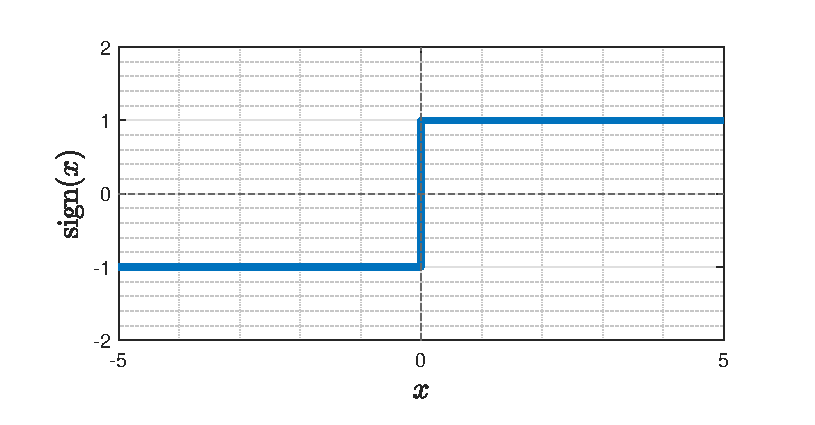
\includegraphics[width=\textwidth]{images/sign.eps}
\end{figure}\end{minipage}
%\end{itemize}
\end{itemize}

\begin{tcolorbox}[breakable]
\underline{\textsc{Example}}\footnote{Example adopted from \textbf{Signals and Systems, 2nd Edition}, P424}\\
A ship encounters the superposition of three wave trains, each of which can be modeled as a sinusoidal signal. 
\[ x(t) = 1+\frac{1}{2}\cos(2\pi t + \phi_{1})+\cos(4\pi t + \phi_{2})+\frac{2}{3}\cos(6\pi t + \phi_{3})\]
With fixed magnitudes for these sinusoids, \textbf{the amplitude of their sum may be quite small or very large, depending on the relative phases.} The implications of phase for the ship, therefore, are quite significant. 
\begin{figure}[H] \centering
\includegraphics[width=0.6\textwidth]{images/phase}
\end{figure}
\end{tcolorbox}

Specifically, for the circuit example above:
\[ \lvert H(\omega_{0}) \rvert =  \frac{1}{\sqrt{1+\omega^{2}(RC)^{2} }} = \frac{1}{\sqrt{1+(\frac{\omega}{\omega_{c}})^{2}}} \]
\[ \angle H(\omega_{0}) = -tan^{-1}(\omega RC) = -tan^{-1}(\frac{\omega}{\omega_{c}})\]


%------------------FT to periodical signals --------------------% 
\ \\
\subsection{Fourier Transform of Periodic Signals}
If $x(t)$ is a periodic signal:
\[ \mathcal{FT} \{ x(t) \} = 2\pi \sum_{k=-\infty}^{+\infty} c_{k} \delta(\omega - k\omega_{0}) \]
where \[ c_{k}=\frac{1}{T} \int_{-\frac{T}{2}}^{+\frac{T}{2}} x(t) e^{-j\frac{2 \pi k}{T} t} dt \]
\begin{tcolorbox}[breakable]
\underline{\textsc{Derivation}}\\
Fourier series of a periodic signal $x(t)$ with period $T$ is:
\[ x(t) = \sum_{k=-\infty}^{+\infty}c_{k}e^{j \frac{2\pi k}{T}t} \quad \text{with} \quad c_{k} = \frac{1}{T} \int_{-\frac{T}{2}}^{+\frac{T}{2}} x(t)e^{-j \frac{2\pi k}{T}t} dt \]
By applying linearity property:
\begin{align*}\begin{split}
 X(\omega) &= \mathcal{FT} \bigg\{ \sum_{k=-\infty}^{+\infty}c_{k}e^{j \frac{2\pi k}{T}t} \bigg\} \\
 &=\sum_{k=-\infty}^{+\infty}c_{k} \ \mathcal{FT}\{ e^{jk\omega_{0} t}\}\\
 &= 2\pi \sum_{k=-\infty}^{+\infty} c_{k} \delta(\omega - k\omega_{0}) 
 \end{split}\end{align*}
\end{tcolorbox}

\subsubsection{Fourier transform of a train of impulses}
%\[ x(t) = \delta(t-T) \quad X(\omega)=e^{-j\omega T} \]
\[ x(t) = \sum_{n=-\infty}^{+\infty} \delta(t-nT) \ \xrightarrow{\mathcal{FT}}\ X(\omega)=\frac{2\pi}{T}  \ \sum^{+\infty}_{k=-\infty} \delta(\omega-k\omega_{0}) \]
\ where \[ \omega_{0}=\frac{2\pi}{T} \]
\begin{tcolorbox}[breakable]
\underline{\textsc{Derivation}}\\
\[ x(t) = \sum_{n=-\infty}^{+\infty} \delta(t-T) \]
From the definition above, $x(t)$ is periodic with period $T$:
\[ x(t) = \sum_{k=-\infty}^{+\infty}c_{k}e^{j \frac{2\pi k}{T}t} \quad \text{with} \quad c_{k} = \frac{1}{T} \int_{-\frac{T}{2}}^{+\frac{T}{2}} \delta(t)e^{-j \frac{2\pi k}{T}t} dt = \frac{1}{T} \]
Thus:
\[ X(\omega) = \frac{2\pi}{T}\sum_{n=-\infty}^{+\infty}  \delta(\omega-k\omega_{0}) \quad  \text{with}\  \omega_{0}=\frac{2\pi}{T}\]
\end{tcolorbox}


%-------------------Sampling theorem---------------------%
\newpage
\section{Sampling Theorem}

To obtain a discrete-time signal from a continuous-time signal, we need a \textbf{C/D converter}.
 \begin{figure}[H]\centering
 \includegraphics[width = 0.4\textwidth]{images/cdconverter}
 \caption{C/D converter} \end{figure}
 \ \\
The mathematical expression for a C/D converter is:
\[ x[n] = x_{c}(nT) \quad -\infty < n < +\infty \]
\ where $T$ is sampling period, $f_{s} = \frac{1}{T}$ is sampling frequency. 
\begin{itemize}
\item In general, the C/D transformation cannot be inverted.
\item Infinite continuous signals can reproduce a given sequence of samples,
\end{itemize}
An ideal C/D converter applies $T$ property, so that the sampling can be done without loosing information. 

%-------------------Sampling Process---------------------%
\subsection{Sampling Process}
Impulse train modulator $s(t)$ is: 
\[ s(t) = \sum_{-\infty}^{+\infty} \ \delta(t-nT) \]
The sampled signal $x_{s}(t)$ is obtained by multiplying the impulse train modulator by the continuous-time signal $x_{c}(t)$:
\begin{align*} 
\begin{split}
x_{s}(t) &= x_{c}(t) \ s(t)\\
&= \sum_{n=-\infty}^{+\infty} x_{c}(t) \delta(t-nT)\\
&= \sum_{n=-\infty}^{+\infty} x_{c}(nT) \delta(t-nT)
\end{split}
\end{align*}
Sampled signal, $x_{s}(t)$, is still defined in continuous-time, but it contains all information in the sampled discrete-time domain.\\\\

\begin{minipage}{\textwidth}
\begin{wrapfigure}{r}{0.5\textwidth}
\includegraphics[width = 0.5\textwidth]{images/sampling1}
\caption{(a)Original signal;(b) Sampled signal } \end{wrapfigure}
Apply the Fourier transform to  $x_{s}(t)$:
\begin{align*} \begin{split}
X_{s}(\omega) &= \mathcal{FT}\{x_{c}(t)\} \cdot \mathcal{FT}\{s(t)\}\\
&=\frac{1}{2\pi} X_{c}(\omega) * \mathcal{FT}\{s(t)\} \\
&=\frac{1}{T} X_{c}(\omega) * \sum_{n=-\infty}^{+\infty} \delta (\omega - k \omega_{s})\\
&=\boxed{\frac{1}{T} \sum_{n=-\infty}^{+\infty}  X_{c}(\omega - k \omega_{s})}
\end{split} \end{align*}
where sampling frequency $\omega_{s}=\omega_{0}=\frac{2\pi}{T}$.
\end{minipage}
\ \\\\\\
For sampled signals: $\omega_{N}$ is the signal bandwidth
\begin{itemize}
\item if $\omega_{s} \geq 2\omega_{N}$, the replicas in the periodization do not overlap
\item if $\omega_{s} < 2\omega_{N}$, the replicas overlap, also known as aliasing\footnote{In Latin, "alias" means "others"}.
\end{itemize} 

\begin{figure}[H]\centering
\includegraphics[width = 0.6\textwidth]{images/sampling2}
\caption{(c) $\omega_{s} \geq 2\omega_{N}$; \ (d) aliasing: $\omega_{s} < 2\omega_{N}$} \end{figure}

%-------------------Reconstruction Process---------------------%
\subsection{Reconstruction Process}
Ideal low-pass filters can be used to reconstruct the signals.
\begin{figure}[H]\centering
\includegraphics[width = 0.5\textwidth]{images/lowpass}
\caption{Low-pass filter system} \end{figure}

\begin{figure}[H]
\begin{minipage}{0.6\textwidth}
1. Multiply the sampled signals by the function $H_{r}(\omega)$ \\
\[ X_{c}(\omega) = X_{s}(\omega) \cdot H_{r}(\omega) \]
\end{minipage} \hfill
\begin{minipage}{0.5\textwidth}
\includegraphics[width = \textwidth]{images/homega}
\caption{$H_{r}(\omega)$}
\end{minipage}\end{figure}

\begin{figure}[H]
\begin{minipage}{0.65\textwidth}
2. Due to the convolution property:
\[ X_{c}(\omega) = \mathcal{FT} \{  x_{s}(t) * h_{r}(t) \} \]
3. Apply inverse Fourier transform:
\begin{align*} \begin{split}
 x_{c}(t)&= x_{s}(t) * h_{r}(t) \\
 &=\sum_{n=-\infty}^{+\infty} x_{c}(nT) \delta(t-nT) * h_{r}(t)\\
 &=\boxed{\sum_{n=-\infty}^{+\infty} x_{c}(nT) h_{r}(t-nT)}\\\\
 &=\sum_{n=-\infty}^{+\infty} x_{c}(nT) \frac{\sin(\pi(t-nT) / T)}{\pi(t-nT) / T}
\end{split}\end{align*}
with \[ h_{r}(t)=\frac{\sin(\pi t/T)}{\pi t/T} \]
\end{minipage} \hfill
\begin{minipage}{0.35\textwidth}
\includegraphics[width = \textwidth]{images/reconstruction2}
\caption{Reconstruction}
\end{minipage}
\end{figure}
%\begin{align*}%\begin{split}
%x_{c}(t) &= \sum_{n=-\infty}^{+\infty} x_{c}(nT) h_{r}(t-nT)\\
%&=\sum_{n=-\infty}^{+\infty} x_{c}(nT) \frac{\sin(\pi(t-nT) / T)}{\pi(t-nT) / T}
%\end{split} %\end{align*}

%-------------------Nyquist-Shannon Sampling Theorem---------------------%
\subsection{Nyquist-Shannon Sampling Theorem}
Nyquist-Shannon sampling theorem provides the condition under which the C/D transformation \textbf{can be inverted} without loosing information.\\
\begin{tcolorbox}
Let $x_{c}(t)$ be a band-limited signal with $X_{c}(\omega)=0, \ \lvert \omega \rvert \geq \omega_{N}$. Then $x_{c}(t)$ is uniquely determined by its samples $x[n] = x_{c}(nT)$, if 
\[ \omega_{s}=\frac{2\pi}{T} \geq 2\omega_{N} \]
where $2\omega_{N}$ is the minimal sampling rate and referred to as the \textbf{Nyquist rate}.
\\\\
$x_{c}(t)$ can be reconstructed by generating a periodic impulse train in which successive impulses have amplitudes that are successive sample values. This impulse train is then processed through an ideal lowpass filter. The resulting output signal will be exactly equal $x_{c}(t)$.
\end{tcolorbox}
%\newpage
%\section*{Bibliography}
%\begin{table}[H]
%\begin{tabularx}{\textwidth}{c c}
%[1] & Oppenheim, A.V., Willsky, A.S. \& Nawab.S.H. (1997) \emph{Signals and Systems}. - 2nd ed. Upper Saddle River, Prentice-Hall, Inc.\\
%\end{tabularx}
%\end{table}
\end{document}